\section{Results}
\label{Results}
%\section{Data Analysis}
%\label{Data Analysis}

\subsection{Flight Data}
%Notes on how to take the results...
%What is being presented: Five plots total, the flight profile for each year, and cumulative dose for each flight.

\begin{figure}[H]
\centering
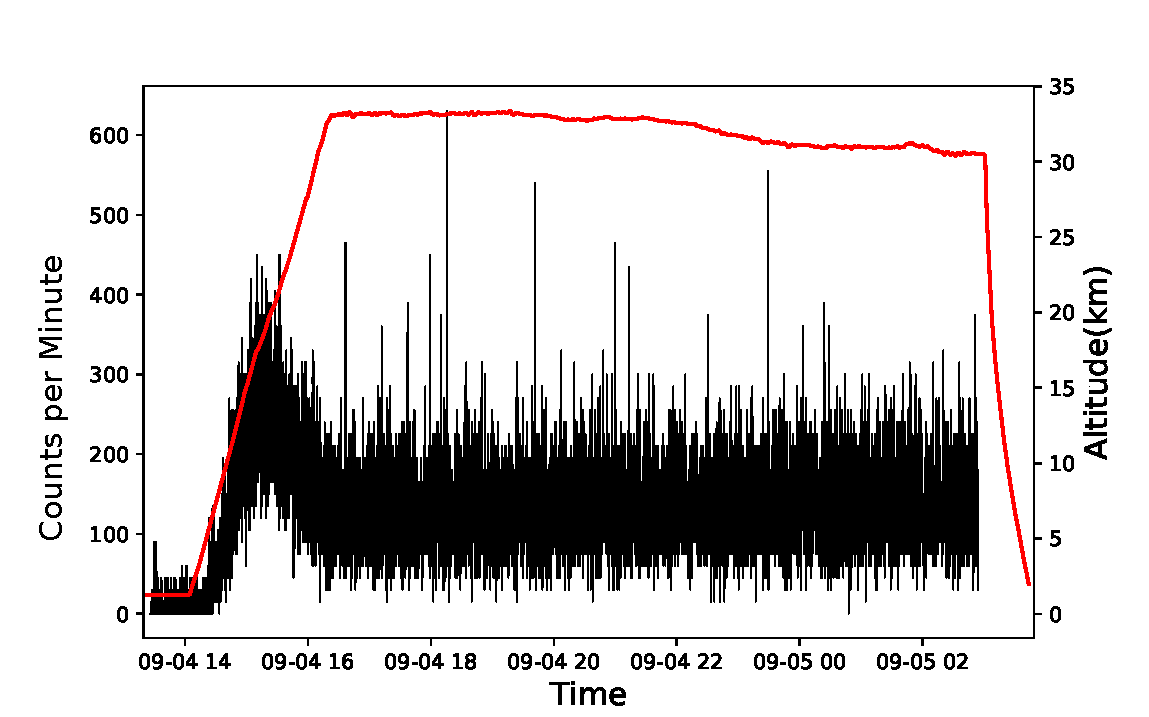
\includegraphics[scale=.75]{count_rate_altitude_2017_f.pdf} %REVIEW 1 from Renshaw: Enlarge this figure and remove the title from the top, titles are not shown in papers since the text and caption should tell you what they are.  Titles are only used in presentations and when sharing the figures around to other people without text or caption. Change the y-axis title to "Counts per Minute"
\caption{Count Rate and Altitude vs Time for 2017 flight. The red line represents the GPS altitude over time in \SI{}{\km}.  The black lines represent the counts per minute over time}
\label{fig:ratealttime_2017}
\end{figure}
%
%First:
%Present and characterize the first two plots - the data of the flight with counts vs altitude vs time.  Here we can talk about each flight and data shown.  Make sure to mention how the count rate changed as time and altitude changed.  We can talk about the flight time, the flight altitude variance, the coasting altitude, and how it all compares to the count rate.  We can be as descriptive as we can.
%mention the position of the pfotzer-regener maximum for both years.  Talk about discrepancies as the data shows.  Speculate in discussion later.
The MiniPIX was set to operate in Time over Threshold mode with a bias voltage of \SI{4}{\kilo\eV}.  Frames were collected at static 4 second intervals during the 2017 flight and between 1 and 4 second intervals for the 2018 flight.  The complete flight altitude profiles and count rates for the SORA  2017 and 2018 flights are shown in Figure~\ref{fig:ratealttime_2017} and Figure~\ref{fig:ratealttime_2018}, respectively.
%
\begin{figure}[H]
\centering
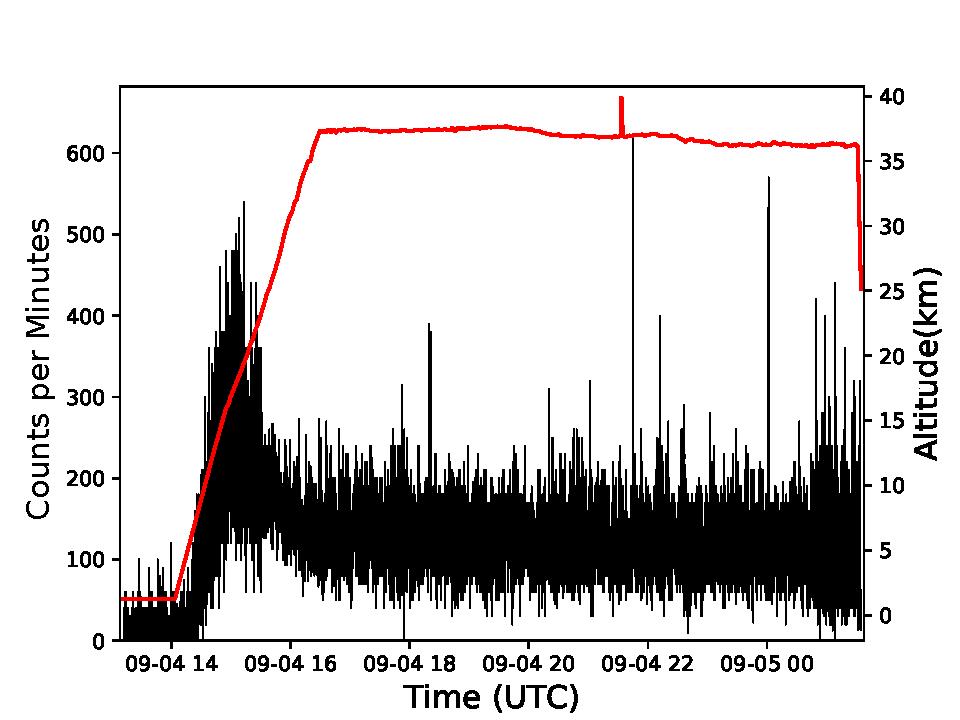
\includegraphics[scale=.80]{count_rate_altitude_2018_f.pdf}%REVIEW 1 from Renshaw: Enlarge this figure and remove the title from the top, titles are not shown in papers since the text and caption should tell you what they are.  Titles are only used in presentations and when sharing the figures around to other people without text or caption. Change the y-axis title to "Counts per Minute"
\caption{Count Rate and Altitude vs Time for 2018 flight. The red line represents the GPS altitude over time in \SI{}{\km}.  The black lines represent the counts per minute over time}
\label{fig:ratealttime_2018}
\end{figure}
%
As shown in Figure~\ref{fig:ratealttime_2017} and Figure~\ref{fig:ratealttime_2018}, both flights have very similar flight altitude profiles.  Both flights reached a float altitude after approximately \SI{2.5}{\hour}.  It is important to mention that the 2017 float altitude was approximately $\SI{31.5}{\kilo\meter}$.  While that for the 2018 flight was about $\SI{37.2}{\kilo\meter}$.  The rate of decent was slow and steady for both flights.  
%
As such, data was collected continuously throughout the whole flights. %%REVIEW 1 from Renshaw: Be careful about making this comment, based on the two figures, we see the altitude go almost to 0 for 2017, but the data stops before this, while for 2018 the plot cuts off the decent and so it is not clear where the data taking stopped.  I think you should rephrase this to say that data was taken during the entire ascent and float periods of both flights and don't mention anything about the decent since it happened much quicker than the ascent and also in a much less controlled manner since the payload was spinning out of control at that point.
%

\begin{figure}[H]%%%REVIEW 1 from Renshaw: You may want to reverse the order of these two plots, since I believe the count rate is the more fundamental quantity and dose rate is something that extends the count rate based on the energy that is deposited.  Also, Change y-axis title to Counts per Minute, it would also be good to enlarge these figures as much as possible without making them take up an entire page.  Remove the titles from each of the plots. Remove this part of the caption, there is no need or it since this information is given in the real caption.
\centering
\begin{subfigure}{.5\textwidth}
  \centering
  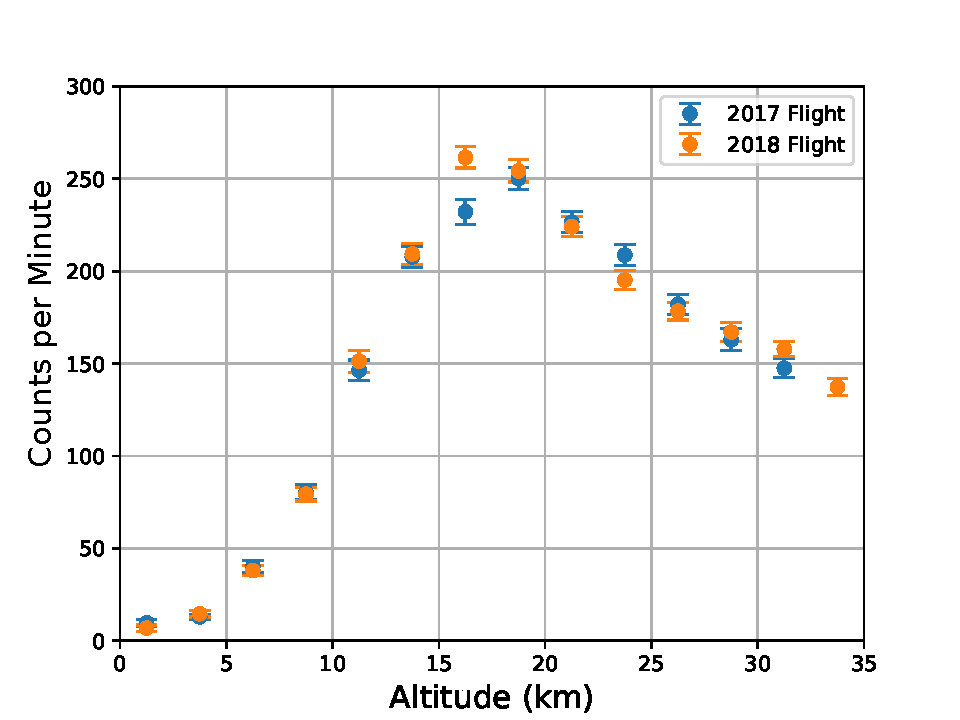
\includegraphics[scale=.45]{cva_stderr_f.pdf}
  \caption{}
  \label{fig:sub2}
\end{subfigure}%
\begin{subfigure}{.5\textwidth}
  \centering
  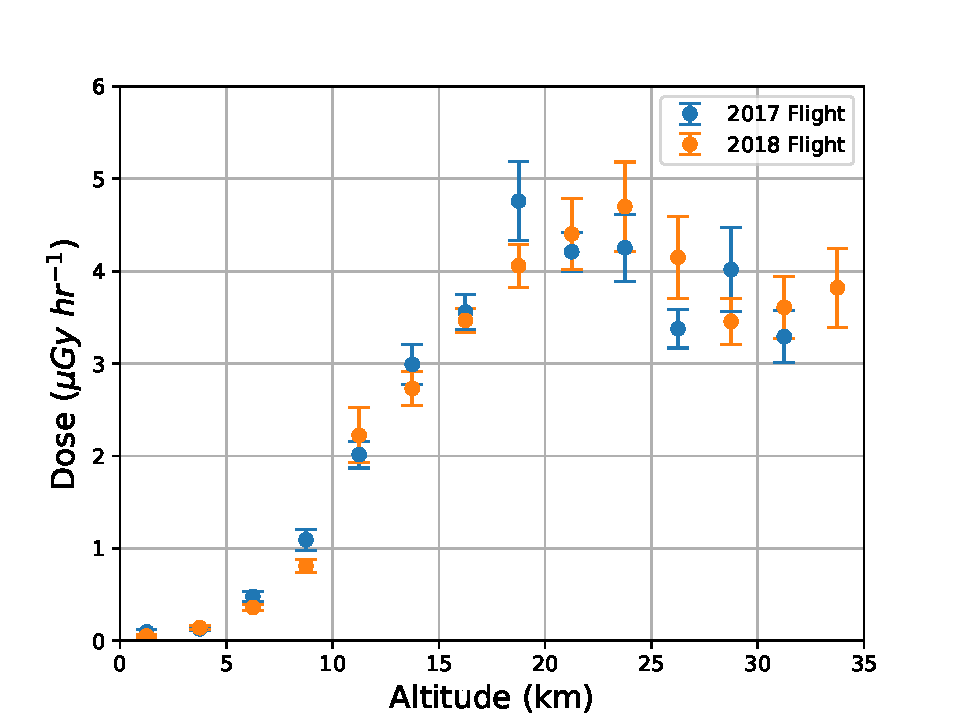
\includegraphics[scale=.45]{dva_stderr_f.pdf}
  \caption{}
  \label{fig:sub1}
\end{subfigure}%
\caption{Figure ~\ref{fig:sub2} shows the detector counts per minute as a function of GPS altitude. Figure ~\ref{fig:sub1} shows the absorbed dose rate in silicon as a function of GPS altitude.  Samples were averaged over \SI{2.5}{\kilo\meter} bins and error bars for both plots represent the standard error of the mean plotted at the $1\sigma$ level.}
\label{fig:dose-count-subplots}
\end{figure}

%% left old here just in case we need to revert
%\centering
%\begin{subfigure}{.5\textwidth}
%  \centering
%  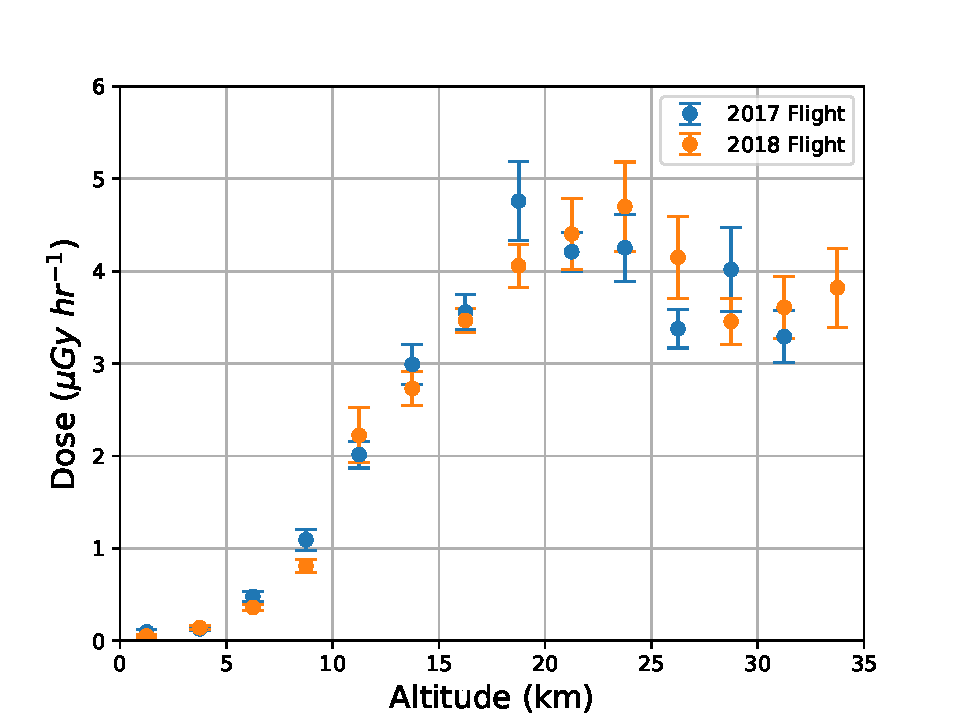
\includegraphics[scale=.45]{dva_stderr_f.pdf}
%  \caption{}
%  \label{fig:sub1}
%\end{subfigure}%
%\begin{subfigure}{.5\textwidth}
%  \centering
%  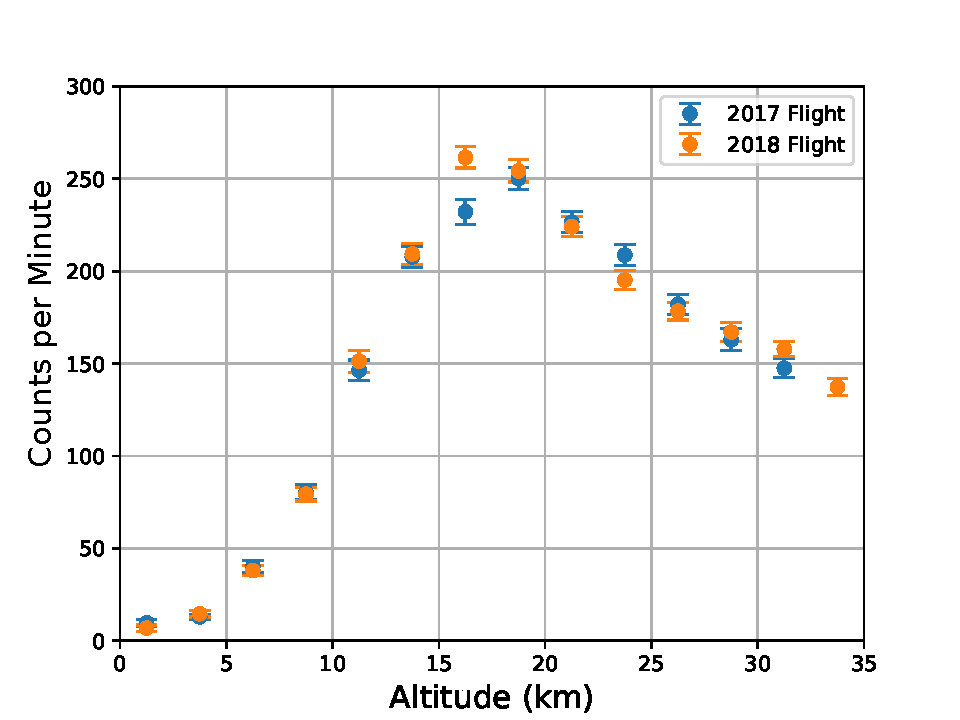
\includegraphics[scale=.45]{cva_stderr_f.pdf}
%  \caption{}
%  \label{fig:sub2}
%\end{subfigure}
%\caption{Figure ~\ref{fig:sub1} shows the absorbed dose rate in silicon as a function of barometric altitude.  Figure ~\ref{fig:sub2} shows the detector counts per minute as a function of barometric altitude. Samples were averaged over \SI{2.5}{\kilo\meter} bins and error bars for both plots represent the standard error of the mean plotted at the $1\sigma$ level.}
%\label{fig:dose-count-subplots}
%\end{figure}
%Next, go into the absorbed rate vs altitude plot.  Mention how the LET varies for materials such as silicon and muscle.  Go into the pfotzer-regener maximum again, compare.  Compare this to the accompanying figure, Detector Hits vs Altitude.  There is a slight discrepancy in the flights, this may be useful to mention.  All error bars are 1 sigma standard deviation.
Shown in Figure~\ref{fig:sub1} and Figure~\ref{fig:sub2} are the dose rate in silicon and the detector count rate plotted as a function of GPS altitude. For the sake of clarity samples were averaged over \SI{2.5}{\kilo\meter} bins and plotted with error bars representing the standard error of the mean at the $1\sigma$ level. Dose rates for both flights appear to be in relatively good agreement up until approximately \SI{16}{\kilo\meter}. After which, the 2017 flight appears to reach a peak dose rate of \SI{4.8}{\micro\gray\per\hour} at approximately \SI{18}{\kilo\meter} while the 2017 flight reaches a peak of \SI{4.8}{\micro\gray\per\hour} at a higher altitude of \SI{24}{\kilo\meter}. 
%
However, the large error bars indicate that it is somewhat unclear as to where the peak dose rate occurs for both flights. %%REVIEW 1 from Renshaw: I would suggest to try and make a fit to the two data series with some function that is taken from a reference which provides the expected rate, this would be a good way to then state what the maximum is and where it is located, with the fit also producing the uncertainty of the location of the max.
%
The dose rates for both flights seem to be in much better agreement than the count rates and show only a small discrepancy between \SI{15}{\kilo\meter} and \SI{17.5}{\kilo\meter} at which the 2018 flight experienced a count rate approximately 30 counts per minute higher than that of the 2017 flight. %%REVIEW 1 from Renshaw:Do we have any idea why this discrepancy is here?  If so it would be good to make a statement about it here. 
%
With both flights reaching altitudes beyond $\SI{25.0}{\kilo\meter}$, the Pfotzer-Regener maximum was clearly observed.  
%
In 2017, the Pfotzer-Regener maximum peaked at approximately  $\SI{18}{\kilo\meter}$.  Similarly, the 2018 mission recorded Pfotzer-Regener maximum peaking around $\SI{20}{\kilo\meter}$. %%REVIEW 1 from Renshaw: Would be good to give the current accepted altitude of the P-R maximum and the reference which states this, then we can directly compare this measurement to that which is accepted 
%
After the observed peaks in count rate, the count rate tapered off inversely with rising altitude.  These count rates then remained constant for the remainder of the flights. %REVIEW 1 from Renshaw: until the float altitude was reached, at which point the count rate remained a constant value, within the uncertainty of the measurement. 

%
%The Pfotzer-Regener maximum is clearly visible between \SI{15}{\kilo\meter} and \SI{20}{\kilo\meter} for both years in both absorbed dose and count rate. 
%
%Variation year over year in measurements of absorbed dose and counts is to be expected and is likely a reflection of the ongoing solar minimum. (need to expand on this a little...)
%
%Another area for the discussion - great area to talk about the discrepancies.  Here we only talk about data and thats it.
%
%Similarly, Figure~\ref{fig:sub2} again confirms the Pfotzer maximum reached for both years.
%For discussion: Here the error is more consistent and Pfotzer maximum is reached at the expected altitudes.

\begin{figure}[H]
\centering
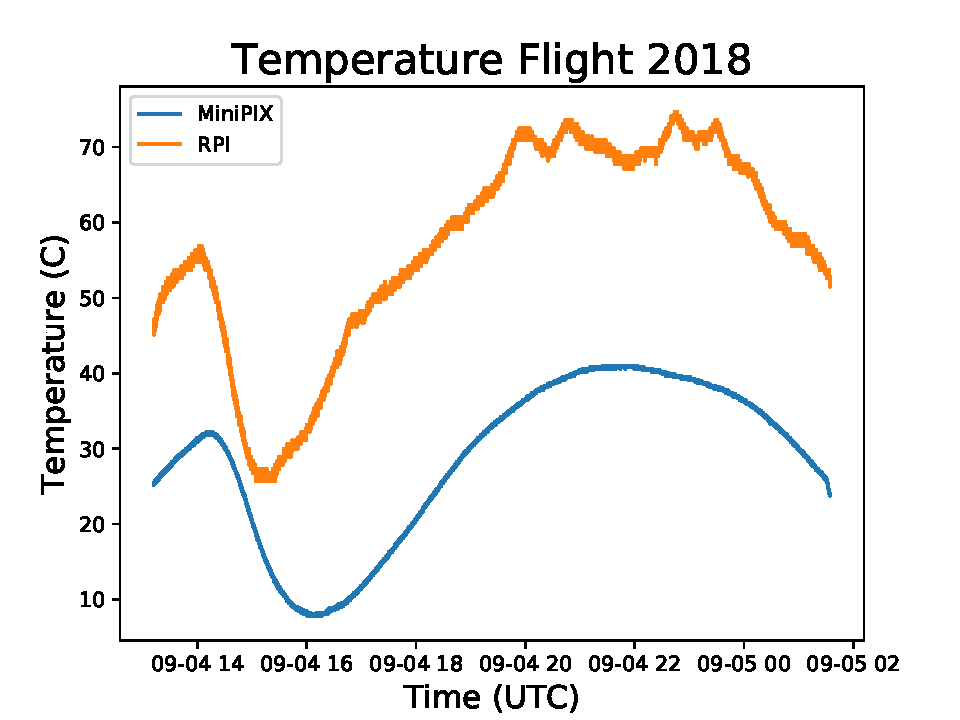
\includegraphics[width=\textwidth]{temps_flight_2018.pdf} %REVIEW 1 from Renshaw: Move this figure and the text associated with it to before the figures and text about the dose rate and count rate. Remove the title from this plot.  Add the degrees symbol to the units for y-axis before the 'C'.
\caption{2018 recorded temperatures of the MiniPIX and Raspberry Pi Flight computer.}
\label{fig:temps_2018}
\end{figure}
%
The MiniPIX and RPI both operated well throughout both flights.  The 2018 flight was better equipped to record system health and operation status.  A key status indicator of system health was the system temperature.  These temperatures recorded are shown in Figure~\ref{fig:temps_2018}.  The MiniPIX temperature stayed within expected ranges and never exceeded $\SI{40}{\degreeCelsius}$.  Likewise, the RPI stayed with operational temperatures.
%FOR Discussion - compare to BEXUS flights and RADX flight as well, and mention how the maximum is similar/different.  Here the maximum in the Hands et al RaD-X mission found the Pfotzer maximum around 60,000 ft (~18 km).  
%
%
%
\begin{figure}[H]
\centering
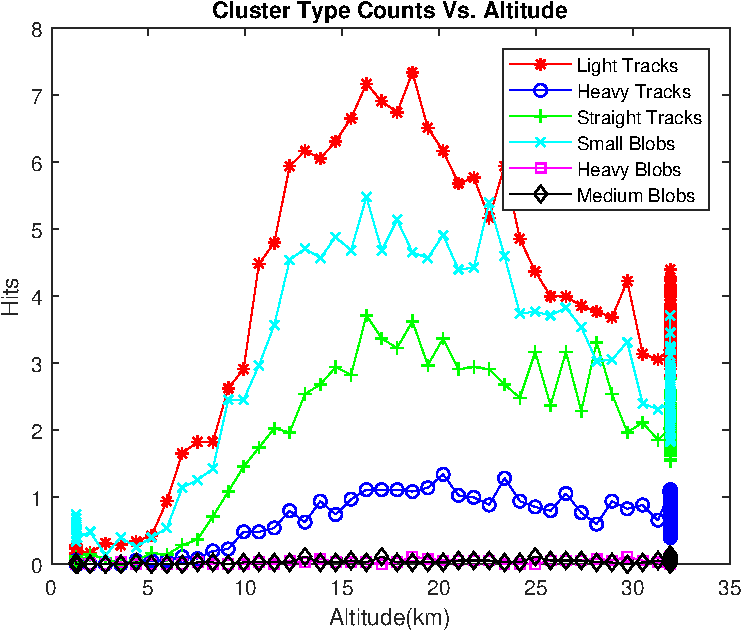
\includegraphics[width=\textwidth]{ctva-cropped.pdf} %% REVEIW 1 from Renshaw: Remove the title from plot.  Make the legend smaller or move it so it does not overlap with the data series.  Put a space between 'Altitude' and '(km)'.  Change y-axis title to 'Number of Hits'. The number of data points at float altitude is confusing and makes the plots hard to read, I would suggest to take an average of these for each data series and then show a single data point for each of them at the float altitude, make sure to take the error bars into account properly when doing the average such that the final error bar represents the spread in the points here
\caption{Distribution of cluster type counts versus altitude for the duration of the 2018 flight.}
\label{fig:cluster2018}
\end{figure}
%Finally, the last figure Cluster Type Counts vs Altitude.  This is useful due to the MiniPIX being able to analyze individual track lengths.  From here, these tracks can be characterized into different and individual categories.  This is useful for LET calculations and overall more precise for dosage calculations.  It may also help with particle identification.
The distribution of cluster types as they vary with altitude is shown in Figure~\ref{fig:cluster2018}.  %%REVIEW 1 from Renshaw: This part needs to be greatly expanded to include the description of what each of the event cluster types are, and then also what type of particles could potentially result in each of the cluster types.  It would also be good to have a figure which shows 6 frames from the MiniPIX, each one giving an example of each of the cluster types so that the reader can see what they actually look like compared to each other.  I imagine that this figure could be laid out in a 2x3 matrix and inserted as a single figure into the paper.
%
%%Sam Changes in response to above review 07/26/12019
%
\begin{figure}[H]
\centering
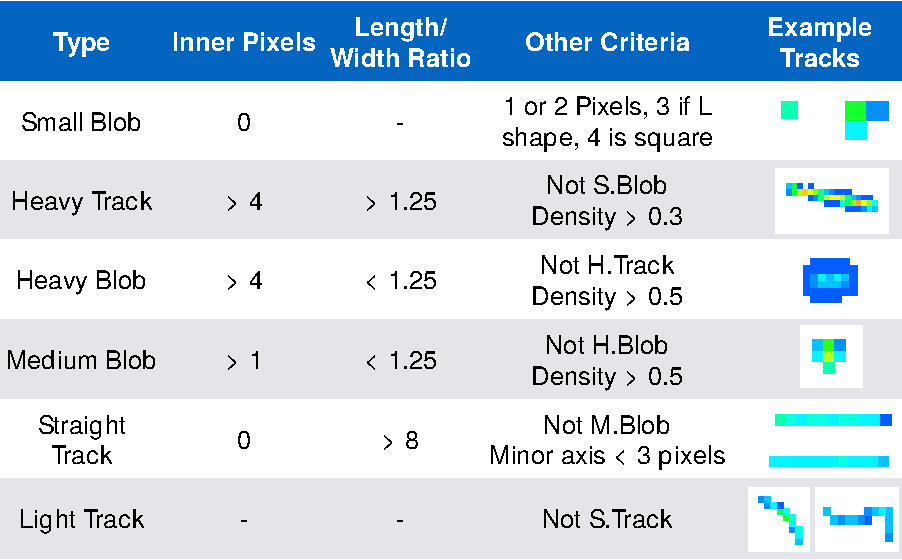
\includegraphics[width=\textwidth]{stuartgraphic.pdf}
\caption{Cluster types CITE ME FROM STUART} %%%NEED CITATION
\label{fig:stuartfigure}
\end{figure}
%
%%End Sam Changes 07/26/2019
%
\begin{figure}[H]
\centering
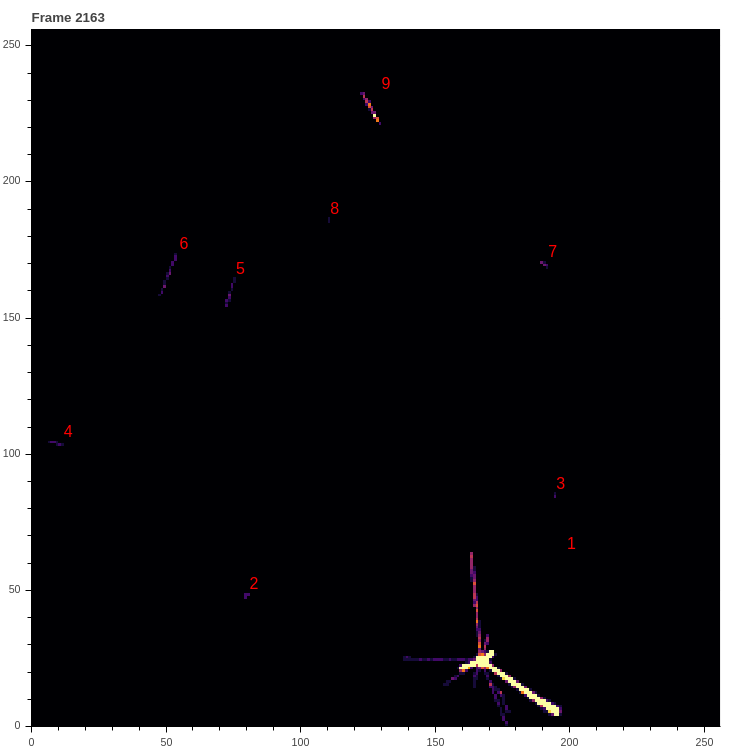
\includegraphics[width=\textwidth]{tracks.png} %No need to give the frame number here, can be removed from the figure and inserted into the caption if you want. It might be good to move this figure and the text for it to before the previous figure and its text, since it would be good to show an example frame and describe that the energy is measured from the track length.  Then show the figure with the different types of clusters, and then the figure with the rate of each of them.  This would be a more logical order in terms of building the understanding for the reader. It would be good to explain this figure better in the text.  So what are each of the numbers in the frame, and why does the large cluster/track look the way it does?
\caption{Single MiniPIX frame collected at float on the 2017 flight.}
\label{fig:frame1}
\end{figure}
Figure~\ref{fig:frame1} shows one of many particle tracks recorded during the 2017 flight, while both flights recorded many frames similar to this.  The track lengths of ionizing particles can be calculated and used to directly measure the linear energy transfer of various primary and secondary particles.


